\chapter{GUIs (Formspecs)}
\label{ch:players/formspecs}

In diesem Kapitel lernst du, wie du eine
Formspec\index{formspec@Formspec} erstellst und dem Spieler anzeigst.
Eine Formspec ist der Beschreibungscode für ein Formular. Formulare sind
in Luanti Fenster wie das Spielerinventar und können verschiedene
Elemente enthalten, etwa Beschriftungen, Schaltflächen und
Eingabefelder.

\begin{figure}
\centering
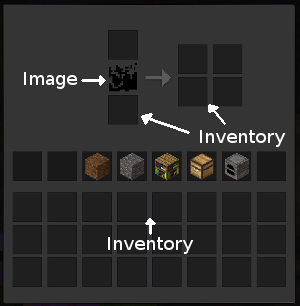
\includegraphics[width=5cm,height=\textheight,keepaspectratio,alt={Formspec eines Ofens mit Beschriftung der Elemente}]{bilder/formspec_example.png}
\caption{Formspec eines Ofens mit Beschriftung der Elemente}
\end{figure}

Musst du keine Eingaben vom Spieler entgegennehmen, sondern ihm nur
Informationen anzeigen, solltest du statt eines Formulars lieber
HUD-Elemente~(Kapitel~\ref{ch:players/hud}) verwenden. Unerwartet
aufgehende Fenster stören nämlich meist das Spiel.

\section{Echte oder alte Koordinaten}\label{echte-oder-alte-koordinaten}

In älteren Versionen von Luanti waren Formspecs uneinheitlich. Elemente
wurden auf unerwartet unterschiedliche Weise positioniert; es war schwer
vorherzusagen, wo sie landen, und sie aneinander auszurichten. Luanti
5.1.0 führte daher \emph{echte Koordinaten} (\emph{real coordinates})
ein, ein einheitliches Koordinatensystem. Echte Koordinaten sind sehr zu
empfehlen, deshalb verwendet dieses Kapitel ausschließlich sie.

Ab \texttt{formspec\_\allowbreak{}version} 2 sind echte Koordinaten
eingeschaltet.

\section{Aufbau einer Formspec}\label{aufbau-einer-formspec}

\subsection{Elemente}\label{elemente}

Formspec ist eine domänenspezifische Sprache mit einem ungewöhnlichen
Format. Sie besteht aus Elementen dieser Form:

\begin{Shaded}
\begin{Highlighting}[]
\NormalTok{typ[param1;param2]}
\end{Highlighting}
\end{Shaded}

Zuerst steht der Elementtyp, dann folgen die Parameter in eckigen
Klammern. Mehrere Elemente können direkt aneinandergehängt oder auf
mehrere Zeilen verteilt werden:

\begin{Shaded}
\begin{Highlighting}[]
\NormalTok{foo[param1]bar[param1]}
\NormalTok{bo[param1]}
\end{Highlighting}
\end{Shaded}

Elemente sind zum Beispiel Textfelder oder Schaltflächen, können aber
auch Metadaten\index{metadaten@Metadaten} wie Größe oder Hintergrund
sein. Eine Liste aller Elemente findest du in der
Lua-API-Referenz\footnote{\url{https://api.luanti.org/formspec/}}.

\subsection{Kopf}\label{kopf}

Der Kopf einer Formspec enthält Angaben, die zuerst stehen müssen: die
Größe der Formspec, ihre Position, den Anker und ob das spielweite Theme
angewendet werden soll.

Die Elemente im Kopf müssen in einer bestimmten Reihenfolge stehen,
sonst gibt es einen Fehler. Diese Reihenfolge ist die im vorigen Absatz
genannte; sie ist, wie immer, auch in der Lua-API-Referenz dokumentiert.

Die Größe wird in Formspec-Feldern angegeben, einer Maßeinheit von
ungefähr 64 Pixeln, die aber je nach Bildschirmdichte und
Skalierungseinstellungen des Clients schwankt. Hier eine Formspec der
Größe \texttt{2,2}:

\begin{Shaded}
\begin{Highlighting}[]
\NormalTok{formspec\_version[4]}
\NormalTok{size[2,2]}
\end{Highlighting}
\end{Shaded}

Beachte, dass wir die Sprachversion der Formspec ausdrücklich angegeben
haben. Ohne sie wird das alte System verwendet, und du kannst weder die
einheitliche Positionierung noch andere neue Funktionen nutzen.

Mit \texttt{position} und \texttt{anchor} platzierst du die Formspec auf
dem Bildschirm. \texttt{position} legt fest, wo auf dem Bildschirm die
Formspec erscheint; Standard ist die Mitte
(\texttt{0.\allowbreak{}5,0.\allowbreak{}5}). \texttt{anchor} legt fest,
welcher Punkt der Formspec an dieser Position liegt; so kannst du sie am
Bildschirmrand ausrichten. Am linken Rand platzierst du die Formspec so:

\begin{Shaded}
\begin{Highlighting}[]
\NormalTok{formspec\_version[4]}
\NormalTok{size[2,2]}
\NormalTok{position[0,0.5]}
\NormalTok{anchor[0,0.5]}
\end{Highlighting}
\end{Shaded}

Damit liegt der Anker in der Mitte des linken Rands der Formspec, und
dieser Anker wird an den linken Bildschirmrand gesetzt.

\section{Ein Ratespiel}\label{ein-ratespiel}

Am besten lernt man, indem man etwas baut. Bauen wir also ein Ratespiel.
Das Prinzip ist einfach: Der Mod denkt sich eine Zahl aus, und der
Spieler rät. Der Mod sagt dann, ob der Tipp zu hoch oder zu niedrig war.

\begin{figure}
\centering
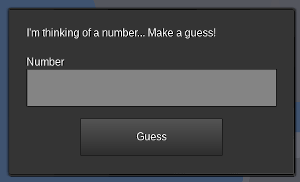
\includegraphics[width=5cm,height=\textheight,keepaspectratio,alt={Die Formspec des Ratespiels}]{bilder/formspec_guessing.png}
\caption{Die Formspec des Ratespiels}
\end{figure}

Zuerst schreiben wir eine Funktion, die den Formspec-Code erzeugt. Das
ist gute Praxis, weil sich der Code so leichter an anderer Stelle
wiederverwenden lässt.

\begin{Shaded}
\begin{Highlighting}[]
\VariableTok{guessing} \OperatorTok{=} \OperatorTok{\{\}}

\KeywordTok{function} \VariableTok{guessing}\OperatorTok{.}\NormalTok{get\_formspec}\OperatorTok{(}\VariableTok{name}\OperatorTok{)}
    \CommentTok{{-}{-} }\AlertTok{TODO}\CommentTok{: anzeigen, ob der Tipp zu hoch/niedrig war}
    \KeywordTok{local} \VariableTok{text} \OperatorTok{=} \StringTok{"Ich denke an eine Zahl ... Rate mal!"}

    \KeywordTok{local} \VariableTok{formspec} \OperatorTok{=} \OperatorTok{\{}
        \StringTok{"formspec\_version[4]"}\OperatorTok{,}
        \StringTok{"size[6,3.476]"}\OperatorTok{,}
        \StringTok{"label[0.375,0.5;"}\OperatorTok{,}
        \VariableTok{core}\OperatorTok{.}\NormalTok{formspec\_escape}\OperatorTok{(}\VariableTok{text}\OperatorTok{),}
        \StringTok{"]"}\OperatorTok{,}
        \StringTok{"field[0.375,1.25;5.25,0.8;number;Zahl;]"}\OperatorTok{,}
        \StringTok{"button[1.5,2.3;3,0.8;guess;Raten]"}\OperatorTok{,}
    \OperatorTok{\}}

    \CommentTok{{-}{-} table.concat ist schneller als Verkettung mit \textasciigrave{}..\textasciigrave{}}
    \ControlFlowTok{return} \FunctionTok{table.concat}\OperatorTok{(}\VariableTok{formspec}\OperatorTok{,} \StringTok{""}\OperatorTok{)}
\KeywordTok{end}
\end{Highlighting}
\end{Shaded}

Hier platzieren wir ein Eingabefeld, eine Beschriftung und eine
Schaltfläche. In das Feld kann man Text eingeben, die Schaltfläche
schickt das Formular ab. Die Elemente sind sorgfältig positioniert, um
Innenabstand und Zwischenraum zu erzeugen; das wird gleich erklärt.

Als Nächstes soll der Spieler die Formspec öffnen können. Der übliche
Weg dafür ist \texttt{show\_\allowbreak{}formspec}:

\begin{Shaded}
\begin{Highlighting}[]
\KeywordTok{function} \VariableTok{guessing}\OperatorTok{.}\NormalTok{show\_to}\OperatorTok{(}\VariableTok{name}\OperatorTok{)}
    \VariableTok{core}\OperatorTok{.}\NormalTok{show\_formspec}\OperatorTok{(}
        \VariableTok{name}\OperatorTok{,}
        \StringTok{"guessing:game"}\OperatorTok{,}
        \VariableTok{guessing}\OperatorTok{.}\NormalTok{get\_formspec}\OperatorTok{(}\VariableTok{name}\OperatorTok{)}
    \OperatorTok{)}
\KeywordTok{end}

\VariableTok{core}\OperatorTok{.}\NormalTok{register\_chatcommand}\OperatorTok{(}\StringTok{"game"}\OperatorTok{,} \OperatorTok{\{}
    \VariableTok{func} \OperatorTok{=} \KeywordTok{function}\OperatorTok{(}\VariableTok{name}\OperatorTok{)}
        \VariableTok{guessing}\OperatorTok{.}\NormalTok{show\_to}\OperatorTok{(}\VariableTok{name}\OperatorTok{)}
    \KeywordTok{end}\OperatorTok{,}
\OperatorTok{\})}
\end{Highlighting}
\end{Shaded}

\texttt{show\_\allowbreak{}formspec} erwartet einen Spielernamen, den
Namen der Formspec und die Formspec selbst. Der Name der Formspec sollte
ein gültiger Itemname sein, also im Format \texttt{modname:itemname}.

\subsection{Innenabstand und
Zwischenraum}\label{innenabstand-und-zwischenraum}

\begin{figure}
\centering
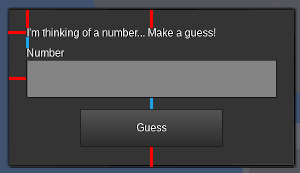
\includegraphics[width=5cm,height=\textheight,keepaspectratio,alt={Innenabstand (rot) und Zwischenraum (blau)}]{bilder/formspec_padding_spacing.png}
\caption{Innenabstand (rot) und Zwischenraum (blau)}
\end{figure}

Der Innenabstand (\emph{padding}, rot) ist der Abstand zwischen dem Rand
der Formspec und ihrem Inhalt oder zwischen Elementen, die nicht
zusammengehören. Der Zwischenraum (\emph{spacing}, blau) ist der Abstand
zwischen zusammengehörenden Elementen.

Üblich sind ein Innenabstand von \texttt{0.\allowbreak{}375} und ein
Zwischenraum von \texttt{0.\allowbreak{}25}.

\subsection{Eingaben empfangen}\label{eingaben-empfangen}

Beim Aufruf von \texttt{show\_\allowbreak{}formspec} wird die Formspec
zum Client geschickt und dort angezeigt. Nützlich wird sie aber erst,
wenn Informationen vom Client zum Server zurückkommen. Dieser Vorgang
heißt \emph{Formspec field submission}; bei
\texttt{show\_\allowbreak{}formspec} empfängst du die Eingaben mit einem
globalen Callback:\index{callback@Callback}

\begin{Shaded}
\begin{Highlighting}[]
\VariableTok{core}\OperatorTok{.}\NormalTok{register\_on\_player\_receive\_fields}\OperatorTok{(}
    \KeywordTok{function}\OperatorTok{(}\VariableTok{player}\OperatorTok{,} \VariableTok{formname}\OperatorTok{,} \VariableTok{fields}\OperatorTok{)}
        \ControlFlowTok{if} \VariableTok{formname} \OperatorTok{\textasciitilde{}=} \StringTok{"guessing:game"} \ControlFlowTok{then}
            \ControlFlowTok{return}
        \ControlFlowTok{end}

        \ControlFlowTok{if} \VariableTok{fields}\OperatorTok{.}\VariableTok{guess} \ControlFlowTok{then}
            \KeywordTok{local} \VariableTok{pname} \OperatorTok{=} \VariableTok{player}\OperatorTok{:}\NormalTok{get\_player\_name}\OperatorTok{()}
            \VariableTok{core}\OperatorTok{.}\NormalTok{chat\_send\_all}\OperatorTok{(}
                \VariableTok{pname}
                    \OperatorTok{..} \StringTok{" hat "}
                    \OperatorTok{..} \VariableTok{fields}\OperatorTok{.}\VariableTok{number}
                    \OperatorTok{..} \StringTok{" geraten"}
            \OperatorTok{)}
        \ControlFlowTok{end}
    \KeywordTok{end}
\OperatorTok{)}
\end{Highlighting}
\end{Shaded}

Die an
\texttt{core.\allowbreak{}register\_\allowbreak{}on\_\allowbreak{}player\_\allowbreak{}receive\_\allowbreak{}fields}\index{core@\texttt{core}!register_on_player_receive_fields@\texttt{core.\allowbreak{}register\_\allowbreak{}on\_\allowbreak{}player\_\allowbreak{}receive\_\allowbreak{}fields}}
übergebene Funktion wird jedes Mal aufgerufen, wenn ein Spieler ein
Formular abschickt. Die meisten Callbacks müssen den übergebenen
Formularnamen prüfen und abbrechen, wenn es nicht das richtige Formular
ist; manche Callbacks arbeiten aber auch mit mehreren oder allen
Formularen.

Der Parameter \texttt{fields} ist eine Tabelle mit den Werten, die der
Spieler abgeschickt hat, indiziert mit Strings. Benannte Elemente
erscheinen je nach Ereignis unter ihrem eigenen Namen. Manche Elemente,
etwa Schaltflächen, werden nur übermittelt, wenn sie das Ereignis
ausgelöst haben; andere, etwa Eingabefelder, sind immer dabei.

\begin{hinweis}{Bösartige Clients können jederzeit alles schicken}

Vertraue niemals den abgeschickten Daten einer Formspec. Ein bösartiger
Client kann jederzeit alles Mögliche schicken -- selbst wenn du ihm die
Formspec nie angezeigt hast. Prüfe also
Privilegien\index{privileg@Privileg} und stelle sicher, dass der Spieler
die Aktion wirklich ausführen darf.

\end{hinweis}

Die Formspec wird jetzt also zum Client geschickt, und der Client
schickt Informationen zurück. Als Nächstes müssen wir die Zielzahl
irgendwie erzeugen und uns merken und die Formspec abhängig von den
Tipps aktualisieren. Dafür gibt es das Konzept der \emph{Kontexte}.

\subsection{Kontexte}\label{kontexte}

Oft soll
\texttt{core.\allowbreak{}show\_\allowbreak{}formspec}\index{core@\texttt{core}!show_formspec@\texttt{core.\allowbreak{}show\_\allowbreak{}formspec}}
dem Callback Informationen mitgeben, die der Client nicht sehen soll --
etwa, mit welchen Argumenten ein Chatbefehl\index{chatbefehl@Chatbefehl}
aufgerufen wurde oder worum es in dem Dialog geht. Hier ist es die
Zielzahl, die wir uns merken müssen.

Ein Kontext ist eine Tabelle je Spieler, in der Informationen
gespeichert werden. Die Kontexte aller Spieler, die gerade online sind,
liegen in einer lokalen Variablen der Datei:

\begin{Shaded}
\begin{Highlighting}[]
\KeywordTok{local} \VariableTok{\_contexts} \OperatorTok{=} \OperatorTok{\{\}}
\KeywordTok{local} \KeywordTok{function}\NormalTok{ get\_context}\OperatorTok{(}\VariableTok{name}\OperatorTok{)}
    \KeywordTok{local} \VariableTok{context} \OperatorTok{=} \VariableTok{\_contexts}\OperatorTok{[}\VariableTok{name}\OperatorTok{]} \KeywordTok{or} \OperatorTok{\{\}}
    \VariableTok{\_contexts}\OperatorTok{[}\VariableTok{name}\OperatorTok{]} \OperatorTok{=} \VariableTok{context}
    \ControlFlowTok{return} \VariableTok{context}
\KeywordTok{end}

\VariableTok{core}\OperatorTok{.}\NormalTok{register\_on\_leaveplayer}\OperatorTok{(}\KeywordTok{function}\OperatorTok{(}\VariableTok{player}\OperatorTok{)}
    \VariableTok{\_contexts}\OperatorTok{[}\VariableTok{player}\OperatorTok{:}\NormalTok{get\_player\_name}\OperatorTok{()]} \OperatorTok{=} \KeywordTok{nil}
\KeywordTok{end}\OperatorTok{)}
\end{Highlighting}
\end{Shaded}

Nun ändern wir den Code zum Anzeigen so, dass er den Kontext
aktualisiert, bevor er die Formspec anzeigt:

\begin{Shaded}
\begin{Highlighting}[]
\KeywordTok{function} \VariableTok{guessing}\OperatorTok{.}\NormalTok{show\_to}\OperatorTok{(}\VariableTok{name}\OperatorTok{)}
    \KeywordTok{local} \VariableTok{context} \OperatorTok{=}\NormalTok{ get\_context}\OperatorTok{(}\VariableTok{name}\OperatorTok{)}
    \VariableTok{context}\OperatorTok{.}\VariableTok{target} \OperatorTok{=} \VariableTok{context}\OperatorTok{.}\VariableTok{target} \KeywordTok{or} \FunctionTok{math.random}\OperatorTok{(}\DecValTok{1}\OperatorTok{,} \DecValTok{10}\OperatorTok{)}

    \KeywordTok{local} \VariableTok{fs} \OperatorTok{=} \VariableTok{guessing}\OperatorTok{.}\NormalTok{get\_formspec}\OperatorTok{(}\VariableTok{name}\OperatorTok{,} \VariableTok{context}\OperatorTok{)}
    \VariableTok{core}\OperatorTok{.}\NormalTok{show\_formspec}\OperatorTok{(}\VariableTok{name}\OperatorTok{,} \StringTok{"guessing:game"}\OperatorTok{,} \VariableTok{fs}\OperatorTok{)}
\KeywordTok{end}
\end{Highlighting}
\end{Shaded}

Auch der Code, der die Formspec erzeugt, muss den Kontext verwenden:

\begin{Shaded}
\begin{Highlighting}[]
\KeywordTok{function} \VariableTok{guessing}\OperatorTok{.}\NormalTok{get\_formspec}\OperatorTok{(}\VariableTok{name}\OperatorTok{,} \VariableTok{context}\OperatorTok{)}
    \KeywordTok{local} \VariableTok{text}
    \ControlFlowTok{if} \KeywordTok{not} \VariableTok{context}\OperatorTok{.}\VariableTok{guess} \ControlFlowTok{then}
        \VariableTok{text} \OperatorTok{=} \StringTok{"Ich denke an eine Zahl ... Rate mal!"}
    \ControlFlowTok{elseif} \VariableTok{context}\OperatorTok{.}\VariableTok{guess} \OperatorTok{==} \VariableTok{context}\OperatorTok{.}\VariableTok{target} \ControlFlowTok{then}
        \VariableTok{text} \OperatorTok{=} \StringTok{"Hurra, richtig geraten!"}
    \ControlFlowTok{elseif} \VariableTok{context}\OperatorTok{.}\VariableTok{guess} \OperatorTok{\textgreater{}} \VariableTok{context}\OperatorTok{.}\VariableTok{target} \ControlFlowTok{then}
        \VariableTok{text} \OperatorTok{=} \StringTok{"Zu hoch!"}
    \ControlFlowTok{else}
        \VariableTok{text} \OperatorTok{=} \StringTok{"Zu niedrig!"}
    \ControlFlowTok{end}

    \CommentTok{{-}{-} … weiter wie oben}
\KeywordTok{end}
\end{Highlighting}
\end{Shaded}

Es ist gute Praxis, dass \texttt{get\_\allowbreak{}formspec} den Kontext
nur liest und nie verändert. Das hält die Funktion einfacher und
leichter testbar.

Zum Schluss muss der Handler den Kontext mit dem Tipp aktualisieren:

\begin{Shaded}
\begin{Highlighting}[]
\ControlFlowTok{if} \VariableTok{fields}\OperatorTok{.}\VariableTok{guess} \ControlFlowTok{then}
    \KeywordTok{local} \VariableTok{name} \OperatorTok{=} \VariableTok{player}\OperatorTok{:}\NormalTok{get\_player\_name}\OperatorTok{()}
    \KeywordTok{local} \VariableTok{context} \OperatorTok{=}\NormalTok{ get\_context}\OperatorTok{(}\VariableTok{name}\OperatorTok{)}
    \VariableTok{context}\OperatorTok{.}\VariableTok{guess} \OperatorTok{=} \FunctionTok{tonumber}\OperatorTok{(}\VariableTok{fields}\OperatorTok{.}\VariableTok{number}\OperatorTok{)}
    \VariableTok{guessing}\OperatorTok{.}\NormalTok{show\_to}\OperatorTok{(}\VariableTok{name}\OperatorTok{)}
\ControlFlowTok{end}
\end{Highlighting}
\end{Shaded}

\section{Wege zur Formspec}\label{wege-zur-formspec}

Eine Formspec kann auf drei Wegen zum Client gelangen:

\begin{itemize}
\tightlist
\item
  show\_formspec: der oben verwendete Weg; die Eingaben empfängt
  \texttt{register\_\allowbreak{}on\_\allowbreak{}player\_\allowbreak{}receive\_\allowbreak{}fields}.
\item
  Formspecs in Node-Metadaten: Der Node hat eine Formspec in seinen
  Metadaten, und der Client zeigt sie \emph{sofort} an, wenn der Spieler
  rechts klickt. Die Eingaben empfängt die Methode
  \texttt{on\_\allowbreak{}receive\_\allowbreak{}fields}\index{callback@Callback!on_receive_fields@\texttt{on\_\allowbreak{}receive\_\allowbreak{}fields}}
  in der Node-Definition.
\item
  Formspecs im Spielerinventar: Die Formspec wird irgendwann zum Client
  geschickt und sofort angezeigt, wenn der Spieler \texttt{i} drückt.
  Die Eingaben empfängt
  \texttt{register\_\allowbreak{}on\_\allowbreak{}player\_\allowbreak{}receive\_\allowbreak{}fields}.
\end{itemize}

\subsection{Formspecs in
Node-Metadaten}\label{formspecs-in-node-metadaten}

\texttt{core.\allowbreak{}show\_\allowbreak{}formspec} ist nicht der
einzige Weg, eine Formspec anzuzeigen; du kannst Formspecs auch in die
Metadaten eines Nodes~(Kapitel~\ref{ch:map/storage}) schreiben. Truhen
machen das zum Beispiel, damit sie schneller aufgehen -- man muss nicht
warten, bis der Server die Formspec der Truhe schickt.

\begin{Shaded}
\begin{Highlighting}[]
\VariableTok{core}\OperatorTok{.}\NormalTok{register\_node}\OperatorTok{(}\StringTok{"mymod:rightclick"}\OperatorTok{,} \OperatorTok{\{}
    \VariableTok{description} \OperatorTok{=} \StringTok{"Klick mich mit rechts!"}\OperatorTok{,}
    \VariableTok{tiles} \OperatorTok{=} \OperatorTok{\{} \StringTok{"mymod\_rightclick.png"} \OperatorTok{\},}
    \VariableTok{groups} \OperatorTok{=} \OperatorTok{\{} \VariableTok{cracky} \OperatorTok{=} \DecValTok{1} \OperatorTok{\},}
    \VariableTok{after\_place\_node} \OperatorTok{=} \KeywordTok{function}\OperatorTok{(}\VariableTok{pos}\OperatorTok{,} \VariableTok{placer}\OperatorTok{)}
        \CommentTok{{-}{-} Läuft, wenn der Node platziert wird, und setzt}
        \CommentTok{{-}{-} die Formspec in den Metadaten des Nodes.}
        \KeywordTok{local} \VariableTok{meta} \OperatorTok{=} \VariableTok{core}\OperatorTok{.}\NormalTok{get\_meta}\OperatorTok{(}\VariableTok{pos}\OperatorTok{)}
        \VariableTok{meta}\OperatorTok{:}\NormalTok{set\_string}\OperatorTok{(}
            \StringTok{"formspec"}\OperatorTok{,}
            \StringTok{"formspec\_version[4]"}
                \OperatorTok{..} \StringTok{"size[5,5]"}
                \OperatorTok{..} \StringTok{"label[1,1;Erscheint beim Rechtsklick]"}
                \OperatorTok{..} \StringTok{"field[1,2;2,1;x;x;]"}
        \OperatorTok{)}
    \KeywordTok{end}\OperatorTok{,}
    \VariableTok{on\_receive\_fields} \OperatorTok{=} \KeywordTok{function}\OperatorTok{(}
        \VariableTok{pos}\OperatorTok{,}
        \VariableTok{formname}\OperatorTok{,}
        \VariableTok{fields}\OperatorTok{,}
        \VariableTok{player}
    \OperatorTok{)}
        \ControlFlowTok{if} \VariableTok{fields}\OperatorTok{.}\VariableTok{quit} \ControlFlowTok{then}
            \ControlFlowTok{return}
        \ControlFlowTok{end}

        \FunctionTok{print}\OperatorTok{(}\VariableTok{fields}\OperatorTok{.}\VariableTok{x}\OperatorTok{)}
    \KeywordTok{end}\OperatorTok{,}
\OperatorTok{\})}
\end{Highlighting}
\end{Shaded}

So gesetzte Formspecs lösen nicht denselben Callback aus. Um Eingaben
aus Formspecs in Metadaten zu empfangen, musst du bei der Registrierung
des Nodes einen Eintrag
\texttt{on\_\allowbreak{}receive\_\allowbreak{}fields} angeben.

Dieser Callback wird auch ausgelöst, wenn du in einem Feld die
Eingabetaste drückst, was mit
\texttt{core.\allowbreak{}show\_\allowbreak{}formspec} nicht möglich
ist. Dafür lässt sich diese Art von Formular nur durch einen Rechtsklick
auf den Node öffnen, nicht per Programmcode.

\subsection{Formspecs im
Spielerinventar}\label{formspecs-im-spielerinventar}

Die Formspec des Spielerinventars erscheint, wenn der Spieler \texttt{i}
drückt. Ihre Ereignisse empfängst du mit dem globalen Callback; der
Formularname ist dabei \texttt{\textquotedbl{}\textquotedbl{}}.

Es gibt verschiedene Mods, mit denen mehrere Mods gemeinsam das
Spielerinventar anpassen können. Minetest Game verwendet
SFINV\footnote{\url{https://github.com/rubenwardy/sfinv/blob/master/Tutorial.md}}.

\subsection{Jetzt bist du dran}\label{jetzt-bist-du-dran}

\begin{itemize}
\tightlist
\item
  Erweitere das Ratespiel so, dass es sich für jeden Spieler die
  Bestleistung merkt, also mit wie wenigen Tipps er die Zahl erraten
  hat.
\item
  Erstelle einen Node „Briefkasten``, in dem Spieler über eine Formspec
  Nachrichten hinterlassen können. Der Node soll den Namen des
  Platzierenden als \texttt{owner} in den Metadaten speichern und mit
  \texttt{show\_\allowbreak{}formspec} unterschiedlichen Spielern
  unterschiedliche Formspecs zeigen.
\end{itemize}
